\documentclass[12pt]{article}

% preamble begins
\title{CS261 Final Report}
\author{Team 29 \\\\ \textbf{Sylvester Cardorelle},\textbf{Tudor Cismarescu}, \textbf{Ollie Madelin},\\
\textbf{Josh Footman}, \textbf{Joseph Parkins}, \textbf{Anil Kiral}}
\date{March 2017}
\usepackage{graphicx}
\usepackage{listings}
\usepackage{scrextend}
\usepackage{titlesec}
\usepackage{float}
\usepackage[margin=1.2in]{geometry}
%preamble ends


%content begins
\begin{document}
\begin{titlepage}
\maketitle
\centering
\vfill
\vfill

\includegraphics[width=7cm]{logo.png}
\vfill
\vfill
\thispagestyle{empty}
\end{titlepage}
\tableofcontents
\section{Installation Guide/ System Requirements}
	\subsection{Setup}
		\subsubsection{Node}
    \subsubsection{SQL}
    \subsubsection{Angular}
    \subsubsection{Npm Installation}
  \subsection{Running}
\section{User Guide}
  \subsection{Analysis tab}
  \subsection{Live Stream tab}
  \subsection{Historical Data tab}
\section{FAQs}
\section{Research}
  After the analysis and design of the project, our software development team had developed a stronger idea
  of the technologies that would be used to design the system. This section further expands on the decisions and
  research that was made after the first deliverable that allowed us to finalise our choice of technologies.
  \subsection{Front-end}
  We decided as a whole group quite early that the whole application would be web-based rather than a desktop app. This would
  increase the accessibility of the application being cross-browser compatible and mobile friendly. If the client integrated a sufficient
  security system, the system could be accessed from anywhere with a secure internet connection.\newline
  The \textbf{AngularJS} framework was used to build the frontend as planned. We considered other JavaScript frameworks,
  such as \textbf{React}, however we felt that AngularJS was the better choice being a full-fledged MVC (Model-View-Controller) framework.
  As our system is a single page application (SPA) that will update dynamically, AngularJS became a natural choice for our developers.
  \newline
  After this decision was made between the Project Manager and Developers, our front-end developers took the initiative to intensively learn AngularJS using a multitude online resources.
  For example, Codecademy a programming teaching platform was used to learn AngularJS basics, whilst AngularJS Community pages were used to further expand their knowledge.
  \subsubsection{JavaScript Graph Library}
  Deciding on a suitable JavaScript Graph Library was crucial for this project as data visualisation was one of our major non-functional requirements.
  After extensive research we decided to use the \textbf{PlotlyJS} library for the following reasons:
  \begin{itemize}
    \item It generates responsive graphs that are able to scale dynamically on different platforms e.g. desktops, tablets
    \item PlotlyJS is known for use in financial analytics and supports a variety of graphs e.g. candlestick, boxplots
    \item Uses WebGL technology for graph rendering with a speed that surpasses many competitors
    \item Provides the option to export the rendered graphs as PNG files for further inspection if needed
    \item Allows the zooming into of graphs, allowing the user to further inspect specific areas of the graph
  \end{itemize}
  \subsection{Back-end}
    \subsubsection{Server-Side}
    Node.js was used as our interface between the frontend and the Java backend using the Express framework.
    This decision was made by the Back-end developers built on their exisiting skills with JavaScript. Node is extremely fast,
    compiling JavaScript code directly into machine code using Google's V8 engine, this means when facing large volumes of data
    the system will stay responsive due to the way Node handles concurrency. The modules and templates written in node can be easily
    reused throughout the serverside, thus reducing the size of our application and chance of bugs occuring.
    \newline
    Other popular server-side-scripts were considered such as Django and Ruby on Rails but given the unfamiliarity and time
    constraints, we discarded them because they did not fully utilise the current skills of the developers.
    \subsubsection{Database}
    Deciding whether to store stock data into a MySQL database became a frequently debated topic throughout the development of the application.
    If the system integrated a database ; storing the input stream into the database for a reasonable time period, it would allow us to
    select relevant data at will and improve the chance of the system finding potential perpetrators of any malicious anomalies.
    \newline
    Despite this, if the system relied on the database too heavily, a performance bottleneck would occur. Thus, making our system slower and less responsive.
    Our developer's countermeasure to this was to cache the data within Java's abstract data structures and storing a data for a certain amount
    of time then storing historical data within the database that would not be useful in further algorithmic calculations.
    \newline
    Once the Back-end developers had come to a decision that was then agreed between the whole group, both solutions to our data storage problem had
    been implemented with the MySQL database acting as a failsafe.
\section{Design}
  \subsection{User Interface}
    - color scheme
    - font size
    - abstraction
      - simplicity
         we wanted to develop something that did not require a manual essentialy,
         the apps fundamental operation can be grasped by the client with the assumption
         that they are computer literate.
  \subsection{Pseudocode}
    This section explores the type of algorithms that we used to analyse the input stream of data for anomalies.
    \subsubsection{Pump \& Dump}
    Arguably, Pump \& Dump was the most challenging type of price manipulation that we attempted to detect.
    After researching the characteristics of a Pump \& Dump, our team concluded the following about Pump \& Dump:
    \begin{itemize}
      \item A large batch of cancellation orders will occur before the dumping of stocks by a person or group (\textbf{Undetectable with current data set})
      \item A steady increase of stock value from the average, when the pumping state begins (\textbf{Detectable})
      \item A sudden drop in stock value when the dumping of stocks occur (\textbf{Detectable})
    \end{itemize}
    \begin{figure}[H]
    \centering
    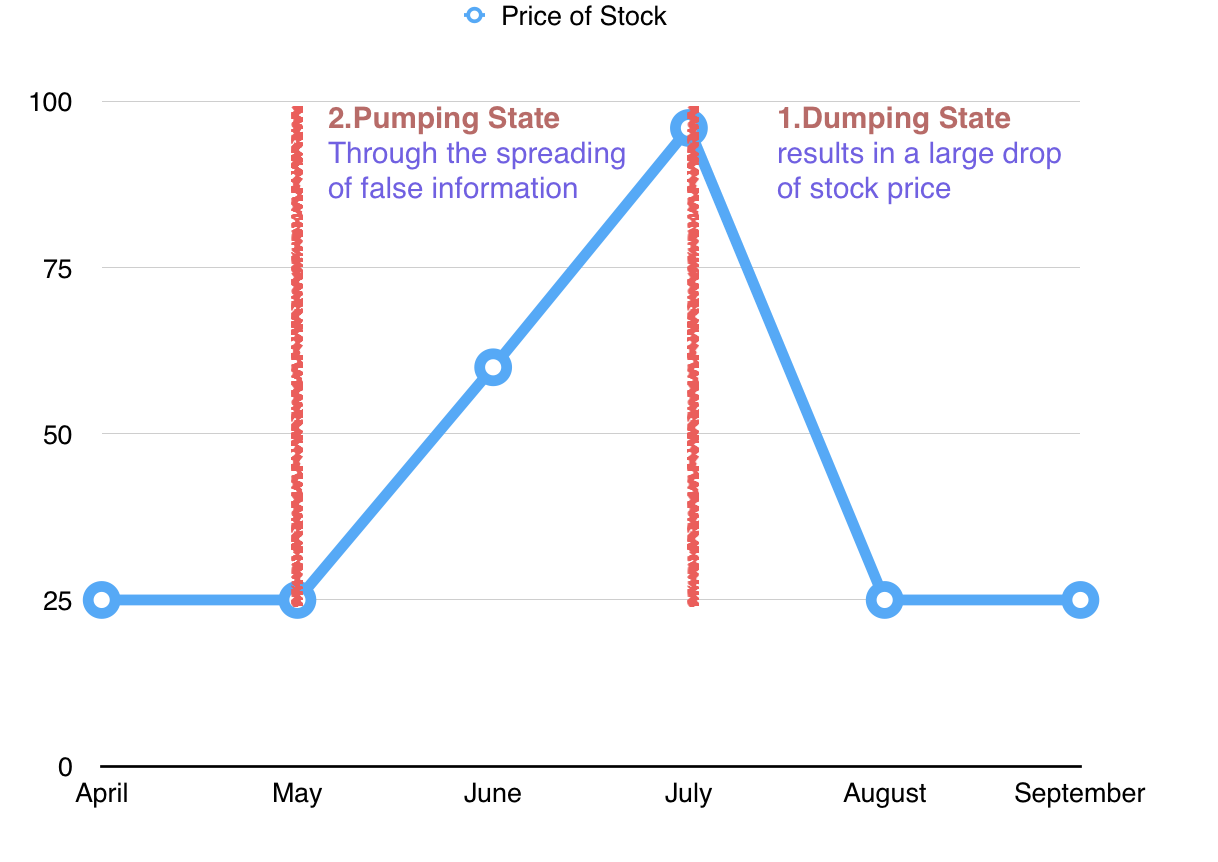
\includegraphics[width=150mm]{PumpDumpGraph.png}
    \caption{Pump \& Dump Example}
    \label{1}
    \end{figure}
    By identifying the traits of a Pump \& Dump, we were able to build the above model in fig:\ref{1}.
    We found it more intuitive to design an algorithm that would first detect a \textbf{dumping state}, then look back
    on historical data to detect whether a \textbf{pumping state} had occured before the drop in stock value. Below in fig:\ref{2} is the
    pseudocode that would later be transformed into Java code.
    \begin{figure}[H]
    \centering
    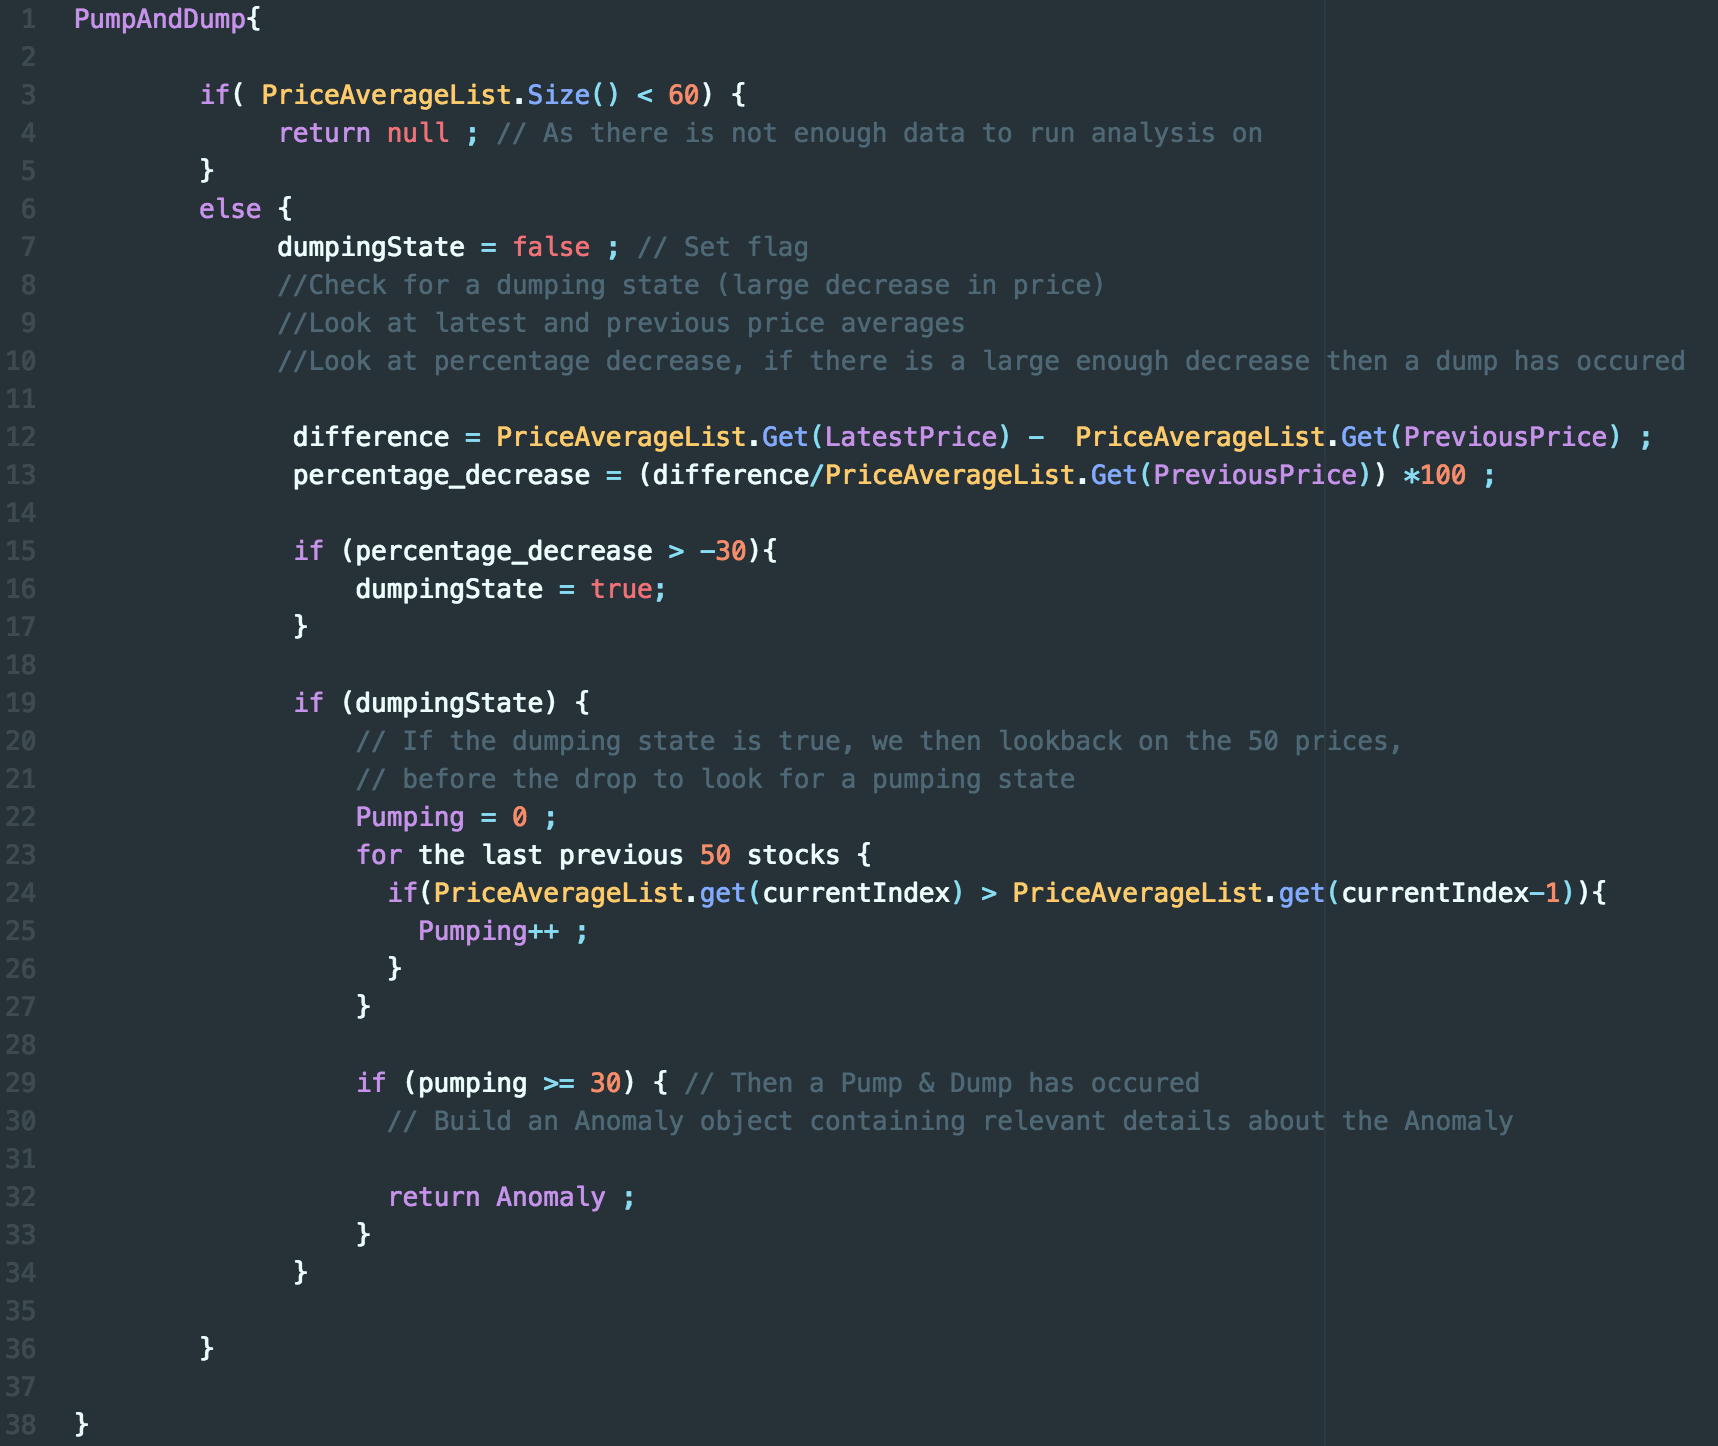
\includegraphics[width=150mm]{PDpseudo.png}
    \caption{Pump \& Dump Pseudocode}
    \label{2}
    \end{figure}
    \subsubsection{Volume Spike}
    To detect volume spikes, we had to keep track of the amount of stocks bought within a certain time interval and compare it to the consequent interval.
    
    \subsubsection{Fat Finger Errors}
\newpage
\section{Implementation}
  \subsection{Frontend}
  \subsection{Backend}
    \subsubsection{Parsing}
\section{Iterations}
  \subsection{Iteration 1}
  \subsection{Iteration 2}
  \subsection{Iteration 3}
  \subsection{Iteration 4}
  \subsection{Iteration 5}
\section{Testing}
  \subsection{Unit Testing}
    \subsubsection{Angular Dependency Injection}
  \subsection{Integration Testing}
  \subsection{System Testing}
  \subsection{User Acceptance Testing}
    \subsubsection{Email Correspondence}
\section{Project Management}
  \subsection{Overview}
  \subsection{Roles}
\section{Evaluation}
\end{document}
% Content ends
